%\documentclass[a4paper,10pt]{article}
\documentclass[11pt,onecolumn]{article}
\usepackage[utf8]{inputenc}
\usepackage[spanish]{babel}
\usepackage{graphicx}
\usepackage{amsmath, amsthm, amsfonts}
\usepackage{listings, color}
\usepackage{float}
\usepackage{longtable}
\usepackage{multicol}
\usepackage{wrapfig}
\usepackage{epstopdf}
\usepackage[right=2.5cm,left=2.5cm,top=2.5cm,bottom=2.5cm,headsep=1cm,footskip=2cm]{geometry}
\usepackage{subfigure}
\usepackage{makeidx}
\usepackage{multirow}




%%%%%%%%%%%%%%%%%%%%%%%  Numero de la experiencia %%%%%%%%%%%%%%
\newcommand{\NUMExp}{4}

\pagestyle{myheadings}

\markboth{Informe \NUMExp{}}{Informe Previo Experiencia \NUMExp{} Laboratorio de Comunicaciones}

\newcommand{\HRule}{\rule{\linewidth}{0.5mm}}

\definecolor{dkgreen}{rgb}{0,0.6,0}
\definecolor{gray}{rgb}{0.5,0.5,0.5}
\definecolor{mauve}{rgb}{0.58,0,0.82}
\definecolor{lgray}{rgb}{0.99,0.97,0.95}
 


\begin{document}
\begin{titlepage}
\setlength{\unitlength}{1 cm}
\thispagestyle{empty}
\begin{picture}(20,0)
\put(12,-1.3){
\includegraphics[scale=0.65]{img/logoelo.pdf}}
\put(-0.1,-2){
\includegraphics[scale=0.10]{img/Logo_utfsm.pdf}}
\end{picture}
\begin{center}


% Upper part of the page
\quad\\[2 cm]
\textsc{\large \ \\ \ Laboratorio de Comunicaciones}\\[2.3 cm]

\textsc{\Large Informe Previo Experiencia \NUMExp{}}\\[0.5cm]


% Title
\HRule \\[0.4cm]
{ \huge \bfseries Reflectometría en el dominio del tiempo y adaptación de impedancias en líneas de transmisión }\\[0.4cm]

\HRule \\[5.7cm]

\begin{table}[h]
\begin{center}
\begin{tabular}{l p{12cm}}
\textbf{\large~Profesor} & \large~ Milan Derpich\\ [0.3cm] 
\textbf{\large~Integrantes} & \large~Roberto Farías \ 201021034-0 \\ [0.1cm] 
\textbf{\large~} & \large~Crsitóbal Ramírez \ 201021030-8 \\ [0.1cm] 
\textbf{\large~} & \large~Crsitóbal Badilla \ 201004063-1 \\ [0.3cm] 
\textbf{\large~Grupo} & \large~3\\ [0.3cm]
\textbf{\large~Fecha} & \large~\Today\\ [0.3cm]
\textbf{\large~Versión} & \large~1.0\\ [0.1cm]

\end{tabular}
\end{center}
\end{table}


\quad\\[1cm]

\vfill

% Bottom of the page
%{\large \today}

\end{center}

\end{titlepage}
\tableofcontents

\newpage
%\listoffigures

%\listoftables
\newpage


%%%%%%%%%%%%%%%%%%%%%%%%INTRODUCCIÓN%%%%%%%%%%%%%%%%%%%%
\newpage 
\section{Resumen}


\section{Objetivos}

\begin{itemize}
\item Simulación de modulación 

\end{itemize}


%%%%%%%%%%%%%%%%%%%%%%%%%%% Desarrollo%%%%%%%%%%%%%%%%%%%%%%%

\newpage
\section{Desarrollo de la Experiencia}

%%%%%%%%%%%%%%PREVIO%%%%%%%%%%%%%%%%%%%%%%%
%\subsection{Trabajo Previo}
% \subsubsection{Simulación controlador PI}
\subsection*{Pregunta 1: Esquema de medición mediante RDT}

La `Reflectometría en el dominio del tiempo' es una técnica que  utiliza el coeficiente de reflexión en líneas de transmisión para obtener los parámetros que infieren en el comportamiento de una línea de transmisión, como lo es su Largo $L$, Largo eléctrico $L_{E}$, velocidad de propagación $v_{p}$, impedancia característica $Z_{0}$, entre otras. Además esta técnica es usada para detectar fallas en lineas de transmisión. Para ello es que se trabaja generalmente en situaciones de cortocircuito y circuito abierto debido a que se conocen las respuestas de reflexión para cada caso.

\begin{wrapfigure}{r}{0.45\textwidth}
  \begin{center}
    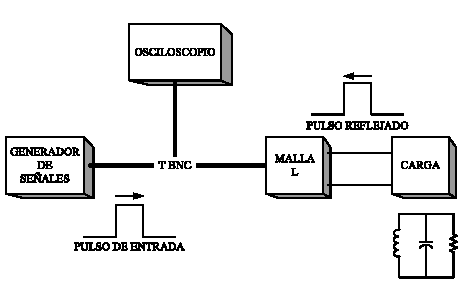
\includegraphics[scale = 1]{img/schema.pdf}
  \end{center}
  \caption{Esquema de medición RDT}
  \label{fig:schrdt}
\end{wrapfigure}

Hay diferentes tipos de reflectómetros, desde un osciloscopio de 
muestro con muy elevado tiempo de respuesta y amplio ancho de banda del orden de los 
GHZ a instrumentos portátiles para detectar fallas en cables. 

Un RDT emite un pulso muy corto en el tiempo. Si el conductor es de una impedancia uniforme
y está apropiadamente terminado, el pulso transmitido se absorberá en la terminación final
y no se reflejará ninguna señal de vuelta hacia el RDT. En cambio, si existen
discontinuidades de impedancia, cada discontinuidad creará un eco que se reflejará hacia el
RDT (de ahí su nombre). Los aumentos en la impedancia crean un eco que refuerza el pulso
original, mientras que las disminuciones en la impedancia crean un eco que se opone el
pulso original. El resultado del pulso medido en la salida/entrada al RDT se representa o
muestra como una función del tiempo y, dado que la velocidad de la propagación de la señal
es relativamente constante para una impedancia dada, puede ser leído como una función de la
longitud de cable. Esto es semejante en su funcionamiento al del radar.

\subsubsection*{Metodología}

\begin{itemize}
\item Esperando que la impedancia característica de la linea $Z_{0}$ sea igual a la impedancia del generador $Z_{G}$ se tendrá que al transmitir un pulso, éste lo hará con la mitad de su amplitud inicial $ V(0,0^{+}) = \frac{V_{G}}{2}$. 

\item En el tiempo $t = \frac{\tau}{2}$ el pulso alcanza el otro extremo de la linea y éste es reflejado como $\frac{V_{G}}{2} \cdot \Gamma_{L}$


\item Luego en el tiempo $t = \tau$ la onda reflejada llega a la posición $Z = 0$, y donde si la duración del pulso es adecuada se sumaran las señales incidentes y reflejadas. Es decir $V(0,\tau) = \dfrac{V_{G}}{2} + \dfrac{V_{g}\cdot \Gamma_{L}}{2}$ 

\item luego del tiempo $t = \tau$ no existirán más cambios de señal debido que no existirán reflexiones de ningún tipo superior a este tiempo.

\end{itemize}
<<<<<<< HEAD
\subsection*{Pregunta 2: Parámetros}
ajdslasdfjlzmxcmcv,zxmcvsdfgiojsdfksdgnxn,xmnsdjlskdfjoiesdfkasjdf
akldsjfklasjdflkafsjdoqiwerudsajlfkz,mzx,cvnafjaslkdjfioqewr
=======
Pregunta 3

Esta es la famoza ecuacxion de DIlbert

	$$S = k log(J)$$
	
Con esto se demuestra que badilla se la come

>>>>>>> 80c4ea2e0620839648ede1c99c06b31de46b81f4










%%%%%%%%%%%%%%%CONCLUSIONES%%%%%%%%%%%%%%%%%%%%%%%%%%%%
\newpage
\section{Conclusiones}

Tras el desarrollo de esta experiencia se puede esperar que:
\begin{itemize}
\item asdasdfads

\end{itemize}


\end{document}

